\documentclass[handout]{beamer}
%
%\mode<presentation>
%{
  \usetheme{Copenhagen} %type de présentation
  %\usecolortheme{blue}% couleur

  %\setbeamercovered{transparent} %laisse le texte à paraître en gris
%}
\usepackage[T1]{fontenc}
\usepackage[utf8]{inputenc}
\usepackage{lmodern}
\usepackage[frenchb]{babel}
\usepackage{amsmath}
\usepackage{amsfonts}
\usepackage{amssymb}
\usepackage{cancel}

\frenchspacing

\allowdisplaybreaks %?
\let\Tiny=\tiny %pour enlever message erreur: Font shape `OT1/cmss/m/n? in size <4> not available
                %(Font) size <5> substituted on input line...

%\beamerdefaultoverlayspecification{<+->}


%-----------------------------------------------------------------------------------------------------------------
\title{Solitons et cosmologie\\ ou symétrie et beauté intersidérale}
\subtitle{Conférence du vendredi}
\author{Éric Dupuis}
\institute{Université de Montréal, département de physique des particules}
\date{XX-XX-2014}


%-----------------------------------------------------------------------------------------------------------------

\begin{document}

%titre
\begin{frame}
\titlepage
\end{frame}
%

\section*{}
\begin{frame}
\tableofcontents
\end{frame}



\section{Cosmologie}
\subsection{Cosmologie 101}
\begin{frame}
\frametitle{Cosmologie 101}
\begin{enumerate}
\item Cosmologie: Structure/origine/évolution de l'univers
\item Constantes de couplage, paramètres libres
\item Univers primordial et théorie d'unification (particules)
\item Atteinte du vide: brisure spontanée de symétrie
%image?
\end{enumerate}
\end{frame}


\subsection{Atteinte du vide}
\begin{frame}
\frametitle{Symétries en physique des particules}
\begin{block}{Brisure spontanée de symétrie}
Les lois de la nature peuvent posséder des symétries sans que l'état de vide (fondamental) le soit nécessairement
\begin{enumerate}
\item Boson: Goldstone, Higgs et les jauges
\item Glashow, Salam et Weinberg: $SU(2)xU(1)$ 
\end{enumerate}
\end{block}
Modèle standard permet les associations suivantes:
\begin{block}{Groupes de Lie pour les forces}
\begin{enumerate}
\item nucléaire faible: SU(2)
\item nucléaire forte: SU(3)
\item électromagnétique: U(1)
\end{enumerate}
\end{block}
\end{frame}

\begin{frame}
\frametitle{Ferroaimant de Heisenberg - Dipôles magnétiques sur réseau}
Invariance de H sous rotation\\
\begin{equation*}
H= -J\sum_{i}{\sum_{voisins j}{\vec{S}_i\vec{S}_j}}
\end{equation*} 
$\rightarrow$ État de plus basse énergie: dipôles alignés \\
 \begin{figure}[0.5\textwidth]
   %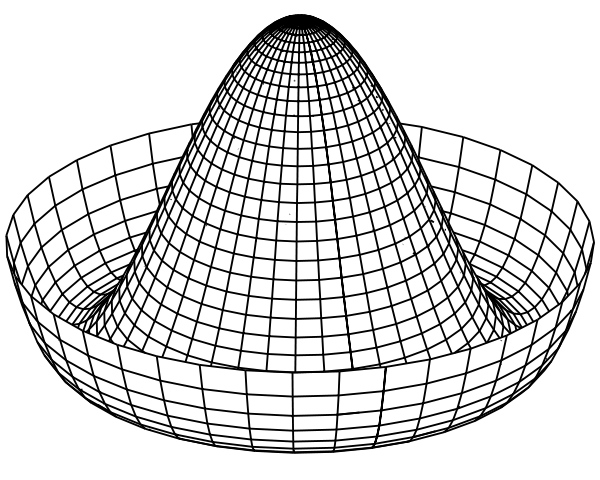
\includegraphics[scale=0.25]{chapeau_mex.png}
   %+ orientés désorientés ou juste tableau?
 \end{figure}

\end{frame}

\begin{frame}
    \begin{figure}[0.3\textwidth]
   %\includegraphics[scale=0.25]{aimants_desorientes.jpg}
    \end{figure}
    Petit homme dans le réseau
    
Et bien plus encore: vortex pour expliquer les supra type I et II
 \end{frame} 

\begin{frame}
\begin{columns}
\begin{column}{.5\linewidth}
    \begin{enumerate}
    \item Température critique (Curie)
    \item Vides dégénérés: défauts topologiques prises (liés au solitons)
   % \item Rencontre: murs de domaine
    %\item $\rightarrow$ murs: liés aux solitons, défauts topologiques
    \end{enumerate}
    \end{column}
	\begin{column}{.5\linewidth}
    \begin{figure}[0.3\textwidth]
    %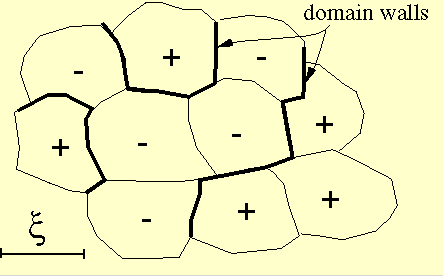
\includegraphics[scale=0.3]{defauts_topo.png}
    \end{figure}
 
	\end{column}
	
\end{columns}
\end{frame}
\subsection{Symétrie et cosmologie}
\begin{frame}

\begin{columns}
    \begin{column}{.5\linewidth}
   \begin{figure}[0.3\textwidth]
    %\includegraphics[scale=0.25]{pot_uni.jpg}
    \end{figure}
    \end{column}
    \begin{column}{.5\linewidth}
    \begin{enumerate}
    \item max: univers primordial (densité d'énergie)
    \item min: notre état de l'univers?
    \item transition, et apparition d'un vrai vide
    \begin{enumerate}
    \item possibilité de transition par effet tunnel
    \item taux de désintégration; dégéneresence des faux vides
    \end{enumerate}
    \end{enumerate}
        %figure Marie-Lou transition du potentiel
    \end{column}
  \end{columns}
  \end{frame}
  
  \begin{frame}
    Symétries brisées spontanément: structure non triviale des vides
    \textbf{Le taux de désintégration de l'univers peut être affecté par la présence de défauts topologiques. Est-ce que l'univers a connu une transition de phase avec brisure de symmétrie? Selon le modèle standard, possiblement. Alors, on attend des cordes cosmiques, monopôles magnétiques. Surtout, ces défauts topologiques pourrait affecter l'évolution actuelle de notre univers. C'est l'objet de notre étude.}
    
  \end{frame}


%-----------------------------------------------------------------------------------------------------------------
\section{Solitons - Appareillage mathématique }

\subsection{Équation d'ondes et soliton}
%eq d'onde
\begin{frame}
\frametitle{Équation d'ondes}
\begin{itemize}
\item  champ scalaire défini dans $\mathbb{R}^n$: $\phi(\vec{x},t)$\\
\end{itemize}
\begin{block}{équation d'onde}
\begin{equation}
\frac{1}{c^2}\frac{\partial^2 \phi}{\partial t^2} - \nabla^2 \phi = \square \phi = 0 
\end{equation}
\textit{Deux propriétés étudiées dans les solutions $\phi$}
\begin{itemize}
\item Forme et vitesse de l'onde conservées\\
\item Deux ondes retrouvent asymptotiquement leur forme et vitesse\\
\end{itemize}
\end{block} 
\end{frame}

%potentiel de solitons
\begin{frame}
\begin{enumerate}
\item Équation d'onde: V=0
\end{enumerate}

\begin{block}{Potentiels différents - Équations du mouvements modifiées}
\begin{enumerate}

\item terme dispersif: $\square\phi +$ \boldmath $m^2 \phi $ \unboldmath  = 0 (Klein-Gordon)\\
\begin{enumerate}
\item onde plane: $k^2 \rightarrow k^2+m^2$

\end{enumerate}
\item terme non-linéaire: $\phi^3$ \\
\end{enumerate}
\end{block}
En s'éloignant de l'équation d'onde, les deux propriétés peuvent être conservées: ondes solitaires et solitons 

\end{frame}

%photo Russell pour le plaisir
\begin{frame}
Sur sa monture, John Russell poursuit sa destinée qui le mène vers l'onde solitaire
\begin{columns}
    \begin{column}{.5\linewidth}
   \begin{figure}[0.3\textwidth]
 %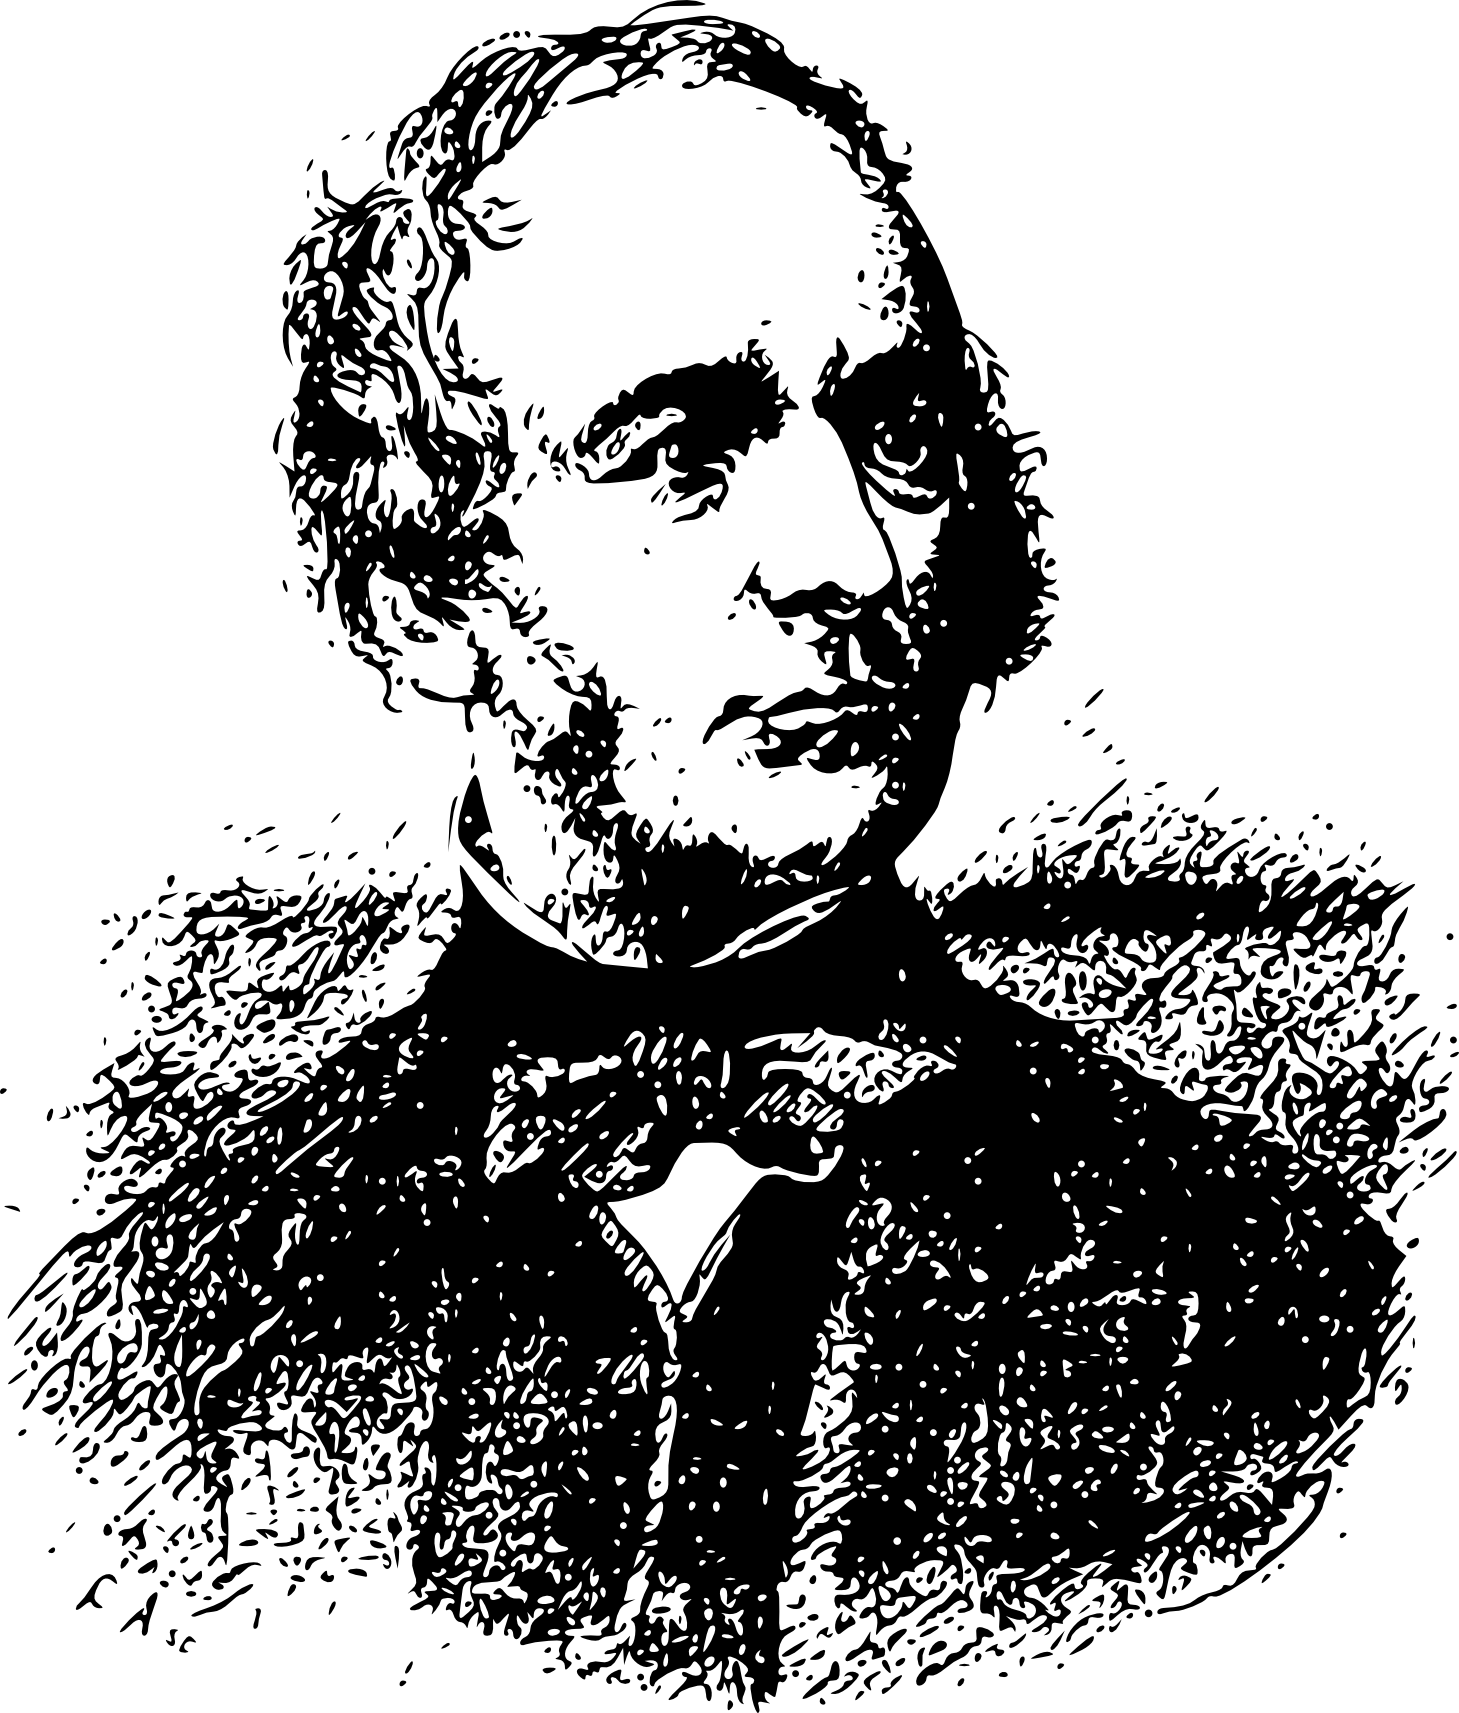
\includegraphics[scale=0.25]{russell.png}
    \end{figure}
    \end{column}
    \begin{column}{.5\linewidth}
    \begin{figure}[0.3\textwidth]
    %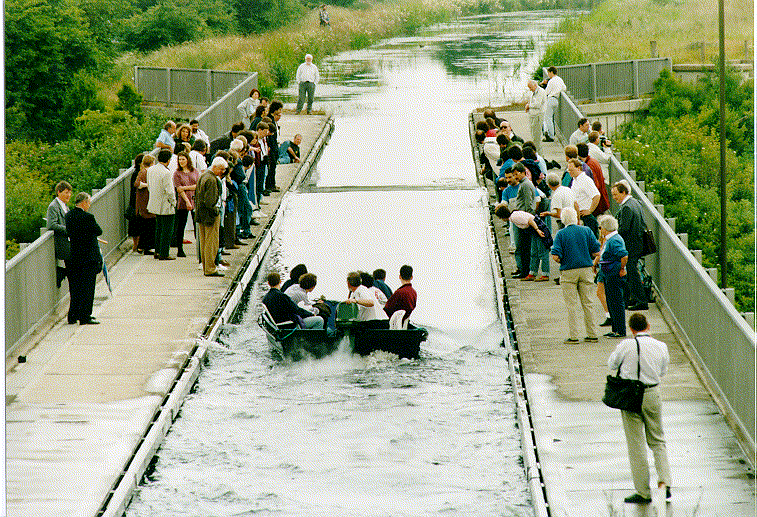
\includegraphics[scale=0.25]{soliton1b.png}
    \end{figure}
    \end{column}
  \end{columns}
\end{frame}


\begin{frame}
	\begin{enumerate}
	\item Densité d'énergie d'un soliton $\epsilon(x,t)$: localisée dans l'espace
	\item $E[\phi] = \int{dxdt (\mathcal{H}[\phi])} = \int{dxdt [\frac{1}{2} \partial_x \phi (\partial_x \phi)^* +V]}$
	\item Énergie finie:
	\begin{enumerate}
	\item  $\lim\limits_{x \to \pm\infty}\partial_x E =0$
	\item  $\lim\limits_{x \to \pm\infty} \phi[x] = g^{(i)}$	
	\end{enumerate}	
	\end{enumerate} 
\end{frame}


\subsection{Formalisme Lagrangien}
\begin{frame}

\frametitle{Formalisme Lagrangien}

\begin{block}{Quelques notions pratiques}
\begin{enumerate}

\item Notation covariante:
\begin{enumerate}
\item $x_0 = ct, x_{1,2,3} = x,y,z$
\item $x^\mu = (x_0,\vec{x})$ et $x^\mu = (x_0,-\vec{x})$
\item Métrique: $x^\mu = g^{\nu\mu} x_\nu$
\item Minkowski: $\eta^{\nu\mu}$ diag(1,-1,-1,-1)
\item indices répétés: $v_a \cdot v_a = \sum_{i=0}^{3}x_i^2$ (produit scalaire)
\end{enumerate}

\end{enumerate}
\end{block}
\end{frame}

\begin{frame}
\begin{enumerate}
\item \textit{Action}: $S[\phi] = \int{dt (L[\phi])}  =  \int{dx_\mu (\mathcal{L}[\phi])}$
\begin{enumerate}
\item Principe d'Hamilton: $\phi_0$ | action minimisée \\
\item Premier ordre nul pour un minimum d'action \\
\end{enumerate}
\item  $\mathcal{L}[\phi] = \frac{1}{2} \partial_\mu \phi (\partial^\mu \phi)^* -V$
\item \textit{Euler-Lagrange:} $\partial_\mu \left(\frac{\mathcal{L}}{\partial(\partial_\mu\phi)}\right) = \frac{\partial\mathcal{L}}{\partial\phi}$
\end{enumerate}
\begin{align*}
 V=0 \\
 \rightarrow (E-L)  \partial_\mu(\frac{\partial_a\phi (\partial^a\phi)^* }{\partial_\mu \phi}) = 0 \\
 \partial_t(\partial^{t} \phi )^{*} + \partial_x(\partial^{x} \phi )^{*} +... = 0 \\
 \square \phi = 0 \\
\end{align*}
\end{frame}

\subsection{Kink}
\begin{frame}
\frametitle{Kink: cas de figure typique}
\begin{block}{Potentiel d'ordre 4}

 \begin{columns}
    \begin{column}{.5\linewidth}
    \begin{enumerate}
    \item deux minimums absolus
    \item ...
	\end{enumerate}      
    \end{column}
    \begin{column}{.5\linewidth}
    $V(\phi) = \frac{\lambda}{4}(|\phi|^2 -\frac{m^2}{\lambda})^2$
    \begin{figure}
     %%\includegraphics[scale=0.5]{boom.jpg}
    \end{figure}
    \end{column}
  \end{columns}

\end{block}
$\mathcal{L} = \frac{1}{2}(\partial_x \phi)^2 - V $ \\
$\rightarrow \phi'' = \lambda \phi^3 - m^2 \phi$ \\
\end{frame}
\begin{frame} \frametitle{Analogie mécanique classique}
\begin{columns}
    \begin{column}{.55\linewidth}
    Champ
    \begin{enumerate}
    \item $\mathcal{H} =  \cancelto{}{\frac{1}{2}  (\partial_t \phi)^2} +  \frac{1}{2}  (\partial_x \phi)^2 +V(\phi) $
    \item $\frac{\partial^2\phi}{\partial_x^2} = \frac{\partial V}{\partial\phi}$
    \item $E_\phi = \int{dx(\frac{1}{2}  (\partial_x \phi)^2 +V(\phi) )}$
    \end{enumerate}
    \end{column}
    \begin{column}{.45\linewidth}
	Particule
    \begin{enumerate}
    \item $L =   \frac{1}{2}  \dot{q}^2 -U(q)$
    \item $\frac{\partial^2\phi}{\partial_x^2} = -\frac{\partial U}{\partial\phi}$
    \item $S_q = \int{dt[\frac{1}{2}  \dot{q}^2 -U(q)] }$
    \end{enumerate}
    \end{column}
  \end{columns}
   \begin{enumerate}
   \item $E_\phi$ finie $\leftrightarrow S_q$ finie $\rightarrow E_q = 0$
   \item On étudie alors: -V
   \end{enumerate}
  
\end{frame}

\begin{frame}
$V(\pm \infty) \rightarrow \pm 1$
\begin{figure}
%%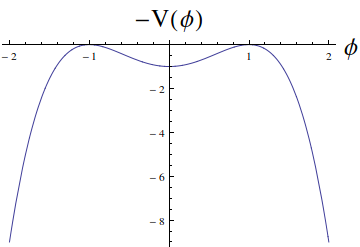
\includegraphics[scale=0.5]{pot_inv.jpg}
\end{figure}
Solution privilégiée: D'un max à l'autre
\end{frame}

\begin{frame}
Récapitulons:
\begin{enumerate}
\item travailler en 1+1 dimensions, mais solution statique
\item Potentiel V $\rightarrow$ Équations d'Euler-Lagrange 
\item $\rightarrow$ équation du mouvement: 
\begin{enumerate}
\item $\rightarrow \phi'' = \lambda \phi^3 - m^2 \phi$ (équation statique)
\item solution: kink
\end{enumerate}
\end{enumerate}
\end{frame}


%-----------------------------------------------------------------------------------------------------------------
\section{Symétrie - Modèles de l'univers }
\begin{frame}

\end{frame}






\section{Quotidien en cosmologie théorique des particules}
\begin{frame}
%potentiel avec lequel on travaille
\begin{block}{Potentiel à deux champs $\phi(x,t)$ et $\psi(x,t)$}
\begin{equation*}
V(\phi,\psi)=(\psi^2-\delta_1)(\psi^2-1)^2+\frac{\alpha}{\psi^2+\gamma}[(\phi^2-1)^2 - \frac{\delta_2}{4}(\phi-2)(\phi+1)^2] 
\end{equation*}
\begin{columns}
    \begin{column}{.5\linewidth}
  
\begin{enumerate}
\item 1+1 dimensions (x,t) mais on cherche une solution statique
\item Beaucoup de paramètres: $\alpha, \gamma, \delta_1, \delta_2$
\item Les champs sont couplés
\end{enumerate}  
    \end{column}
    \begin{column}{.5\linewidth}
    \begin{figure}[0.3\textwidth]
    %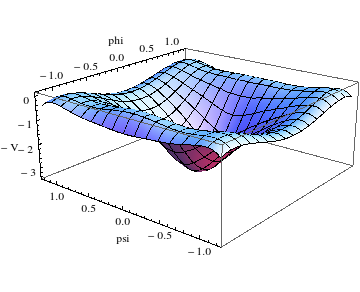
\includegraphics[scale=0.4]{pot2.png}
    \end{figure}
    \end{column}
  \end{columns}
\end{block}
\end{frame}

\begin{frame}
Pourquoi bâtir un potentiel comme ça en premier lieu?!?!\\


\begin{columns}
    \begin{column}{.5\linewidth}
   \begin{figure}[0.3\textwidth]
    % %\includegraphics[scale=0.25]{potpsi.png}
    \end{figure}
   $\delta_1 \rightarrow$ contrôle du minima central\\
    Potentiel d'ordre 6, CLASSIQUE!\\    
    \end{column}
    \begin{column}{.5\linewidth}
    \begin{figure}[0.3\textwidth]
     %%\includegraphics[scale=0.25]{potphi.png}
    \end{figure}
   $\delta_2 \rightarrow$ contrôle de la séparation entre minimum \\
    \end{column}
  \end{columns}
 $\alpha$: importance 2ème terme \\
 $\gamma$: importance couplage \\
\end{frame}

\end{document}